% file: contribution.tex

\documentclass[tikz]{standalone}
\usetikzlibrary{positioning, calc, arrows, arrows.meta, fit}

\begin{document}
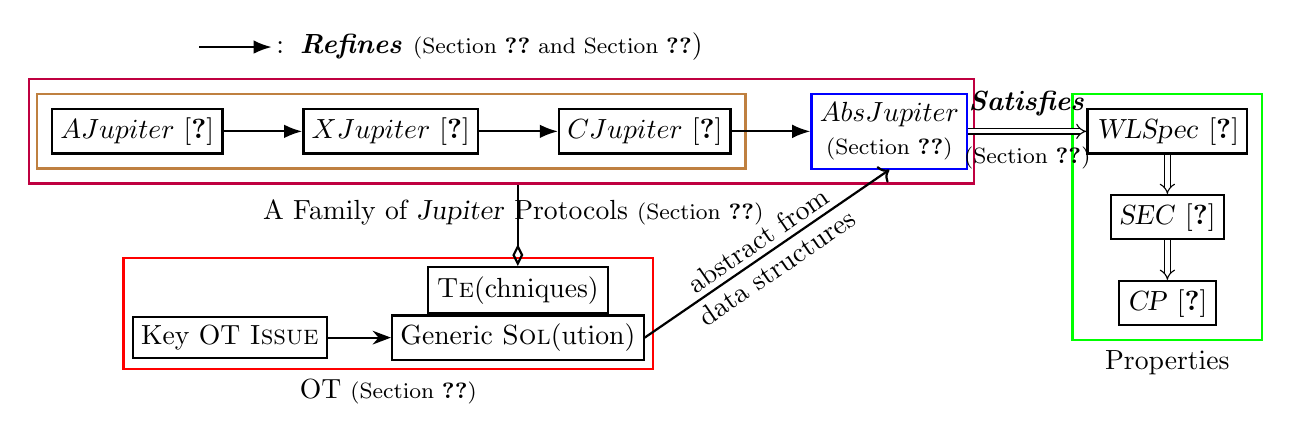
\begin{tikzpicture}[protocol/.style = {draw, thick, inner sep = 3pt},
  ot/.style = {draw, thick, inner sep = 3pt},
  st/.style = {-To, thick},
  spec/.style = {draw, thick, inner sep = 3pt},
  sat/.style = {double equal sign distance, -Implies},
  refine/.style = {>=LaTeX, ->, thick}]
  % jupiter protocols
  \node (aj) [protocol] {$AJupiter$~\cite{Attiya:PODC16}};
  \node (xj) [protocol, right = of aj] {$XJupiter$~\cite{Xu:CSCW14}};
  \node (cj) [protocol, right = of xj] {$CJupiter$~\cite{Wei:OPODIS18}};

  % existing protocols: jupiter variants
  \node (jv) [draw, thick, brown, fit = (aj) (xj) (cj), inner sep = 5pt] {};

  % absjupiter
  \node (absj) [protocol, draw = blue, right = of cj, align = center] {$AbsJupiter$ \\ {\footnotesize (Section~\ref{ss:absjupiter})}};

  % jupiter family
  \node (ajabsj) at ($(aj)!0.5!(absj)$) {};
  \node (jflbl) [below = 18pt of ajabsj] {A Family of \textsl{Jupiter} Protocols {\footnotesize (Section~\ref{section:jupiter-protocols})}};
  \node (jf) [draw, purple, thick, fit = (aj) (absj), xshift = -3pt, inner sep = 5pt] {};

  % ot
  \node (xcj) at ($(xj)!0.5!(cj)$) {};
  \node (sol) [ot, below = 2.2cm of xcj] {Generic \textsc{Sol}(ution)};
  \node (issue) [ot, left = 0.80cm of sol]  {Key OT \textsc{Issue}};

  \draw[-Stealth, thick] (issue) to (sol);

  % ot to jupiter protocols
  % \path (sol) edge[st] (aj)
  %   		  edge[st] (xj)
  %   		  edge[st] (cj)
  %   		  edge[st] (absj);
  \node (st) [draw, thick, above = 0.00cm of sol] {\textsc{Te}(chniques)};
  \node (ot) [draw, thick, red, fit = (issue) (sol) (st), inner sep = 3pt, label = below : OT {\footnotesize (Section~\ref{section:jupiter-family})}] {};
  \draw[{Diamond[open]}-, thick] (st) to (jf.south -| st.north);
  % \draw [>=Stealth] (st) -- (sf);

  % ot to absjupiter
  \draw[st] (sol.east) to node [sloped, align = center] {abstract from \\ data structures} (absj.south);

  % refine
  \path (aj) edge[refine] node (ajrefinexj) {} (xj)
		(xj) edge[refine] node (xjrefinecj) {} (cj)
		(cj) edge[refine] node (cjrefineabsj) {} (absj);
  \node (refinement) [above = 4pt of jf, inner sep = 2pt, label = {left: $:$}] 
	{\textbf{\emph{Refines}} {\footnotesize (Section~\ref{section:refinement} and Section~\ref{ss:tlc-refinement}})};
  \draw[refine, shorten >= 8pt] ($(refinement.west)+(-1.2cm, 0)$) to (refinement);

  % specs
  \node (wlspec) [spec, right = 1.50cm of absj] {\textsl{WLSpec}~\cite{Attiya:PODC16}};
  \node (sec) [spec, below = 0.50cm of wlspec] {\textsl{SEC}~\cite{Shapiro:SSS11}};
  \node (cp) [spec, below = 0.50cm of sec] {\textsl{CP}~\cite{Ellis:SIGMOD89}};
  \node (spec) [fit = (wlspec) (sec) (cp), draw, green, thick, inner sep = 5pt, label = below : Properties] {};

  \draw [sat] (absj) to node [above = 2pt] {\textbf{\emph{Satisfies}}} node[below = 2pt] {\footnotesize (Section~\ref{ss:tlc-correctness})} (wlspec);
  \path (wlspec) edge[sat] (sec)
		(sec) edge[sat] (cp);
  
  % satisfy
  % \node (satisfy) [above = 8pt of spec, inner sep = 2pt, label = {left = -5pt: $:$}] {Satisfies {\footnotesize (Section~\ref{section:tlc-correctness}})};
  % \draw[sat, shorten >= 8pt] ($(satisfy.west)+(-1.2cm, 0)$) to (satisfy);

  % model checking
\end{tikzpicture}
\end{document}
